\documentclass[11pt,a4paper]{article}

\usepackage[margin=1in]{geometry}
\usepackage{graphicx}
\usepackage{booktabs}
\usepackage{hyperref}
\usepackage{float}
\usepackage{subcaption}
\usepackage{array}
\usepackage{enumitem}
\usepackage{xcolor}
\usepackage{titlesec}

\hypersetup{
    colorlinks=true,
    linkcolor=blue,
    urlcolor=blue,
    citecolor=blue
}

\titleformat{\section}{\large\bfseries}{}{0em}{}
\titleformat{\subsection}{\normalsize\bfseries}{}{0em}{}

\newcommand{\course}{AI600 -- Deep Learning}
\newcommand{\assignment}{Assignment 2: Quick, Draw! Challenge}
\newcommand{\studentname}{Muhammad Abdullah}
\newcommand{\rollnumber}{25280050}
\newcommand{\githuburl}{\url{https://github.com/abdull2325/ai600-pa2-25280050}}

\begin{document}

\begin{titlepage}
    \centering
    {\Large Lahore University of Management Sciences\par}
    {\large School of Science and Engineering, Department of Electrical Engineering\par}
    \vspace{1.5cm}

    {\LARGE \textbf{\course}\par}
    \vspace{0.5cm}
    {\Large \textbf{\assignment}\par}
    \vspace{1.8cm}

    \begin{tabular}{>{\bfseries}p{0.30\textwidth} p{0.60\textwidth}}
        Student Name: & \studentname \\
        Roll Number: & \rollnumber \\
        Semester: & Spring 2026 \\
        Submission Date: & \today \\
    \end{tabular}

    \vspace{1.1cm}
    \noindent\fcolorbox{black}{gray!8}{
        \parbox{0.93\textwidth}{
            \textbf{Programming Components (Public GitHub Repository):}\\[2mm]
            \githuburl
        }
    }

    \vfill
    {\large This report documents architecture search experiments under assignment constraints:\\
    no CNNs, parameter budget \(\leq 3{,}000{,}000\), and training budget \(\leq 40\) epochs.\par}
\end{titlepage}

\section{Problem Statement and Constraints}
This assignment uses a 15-class subset of the Quick, Draw! dataset with input bitmaps flattened to 784-dimensional vectors. The objective is to classify doodles using \textbf{only MLP architectures} while respecting:
\begin{itemize}[leftmargin=1.5em]
    \item No convolutional layers.
    \item Maximum trainable parameters: \(3{,}000{,}000\).
    \item Maximum training epochs: \(40\).
\end{itemize}

\section{Data and Training Setup}
\begin{itemize}[leftmargin=1.5em]
    \item Training set: 60,000 labeled samples.
    \item Validation split: 80/20 (48,000 train, 12,000 validation).
    \item Test set: 15,000 unlabeled samples.
    \item Preprocessing: pixel normalization from [0, 255] to [0, 1].
    \item Loss: Cross-Entropy.
    \item Optimizer: AdamW with model-specific learning rates and weight decay.
    \item Regularization strategies explored: dropout, batch normalization, early stopping.
\end{itemize}

\section{Part A/B/C: Architecture Search Results}
Three models were trained as required:
\begin{itemize}[leftmargin=1.5em]
    \item \textbf{Pancake (width-focused):} one wide hidden layer.
    \item \textbf{Tower (depth-focused):} six hidden layers with narrow width.
    \item \textbf{Champion:} tuned depth-width balance for best validation performance.
\end{itemize}

\subsection{Model Configuration Summary}
\begin{table}[H]
\centering
\begin{tabular}{p{0.16\textwidth}p{0.28\textwidth}p{0.14\textwidth}p{0.12\textwidth}p{0.12\textwidth}}
\toprule
Model & Hidden Layers / Width & Params & Used Epochs & Best Val Acc \\
\midrule
Pancake & [2048] & 1,638,415 & 24 & 77.35\% \\
Tower & [256,256,256,256,256,256] & 536,847 & 28 & 78.21\% \\
Champion & [1024,768,512,256] & 2,125,071 & 34 & 79.16\% \\
\bottomrule
\end{tabular}
\caption{Performance and efficiency comparison of the three required models.}
\end{table}

\subsection{Learning Curves}
\begin{figure}[H]
    \centering
    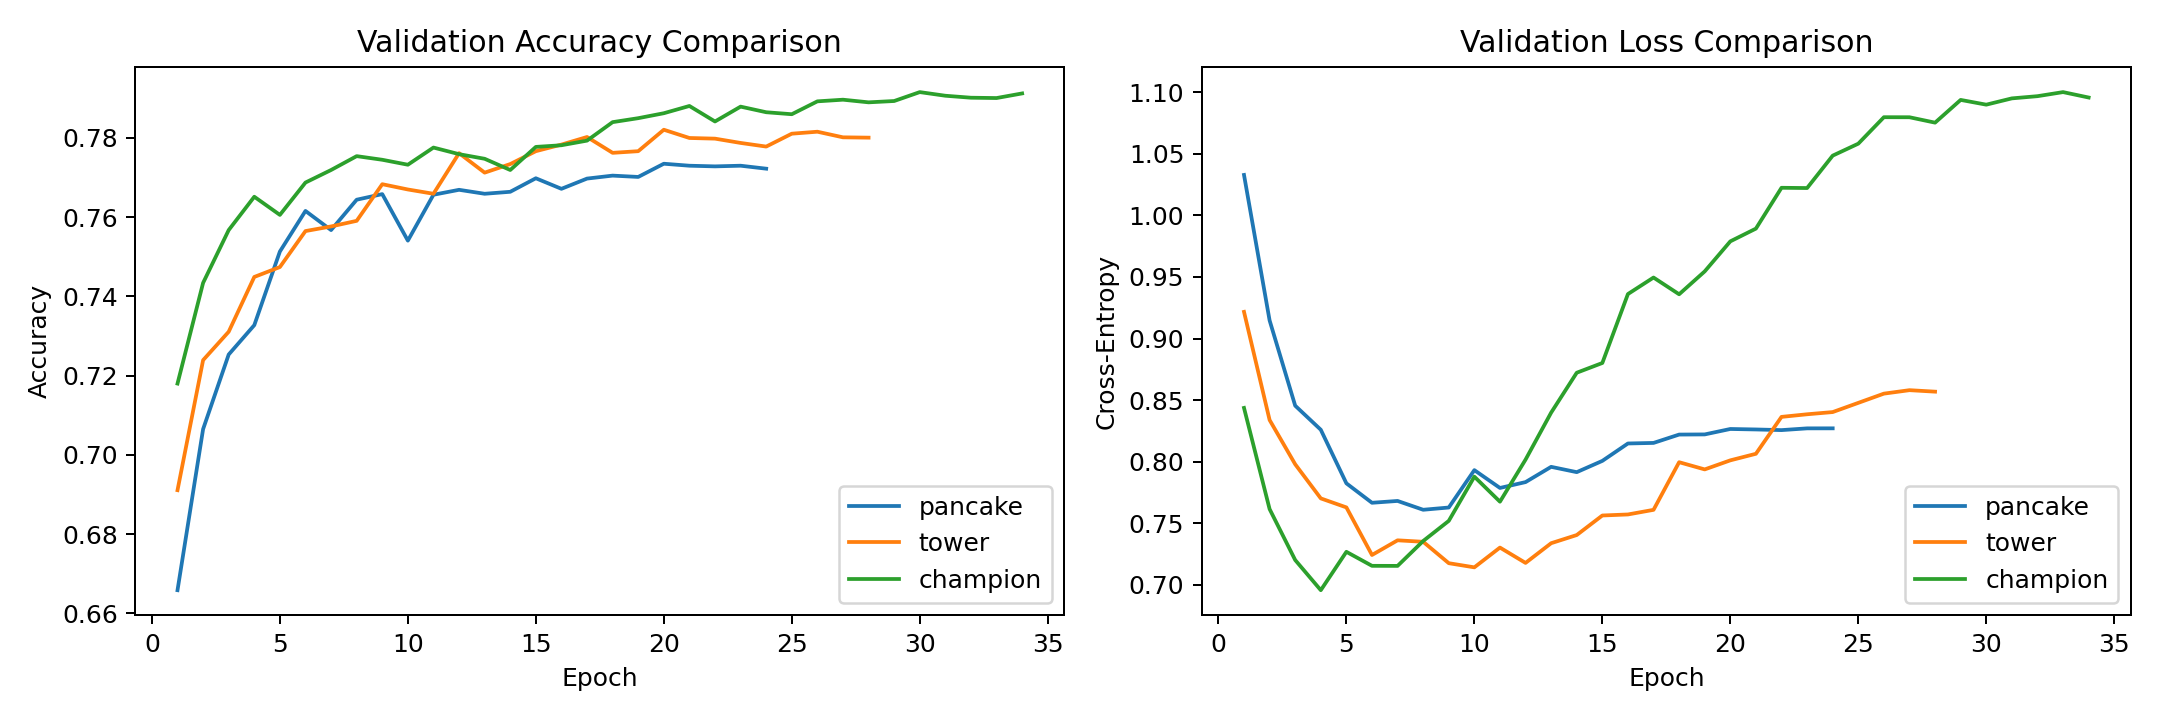
\includegraphics[width=0.95\textwidth]{notebook_outputs/model_comparison.png}
    \caption{Validation accuracy and validation loss comparison across Pancake, Tower, and Champion models.}
\end{figure}

\begin{figure}[H]
    \centering
    \begin{subfigure}[t]{0.48\textwidth}
        \centering
        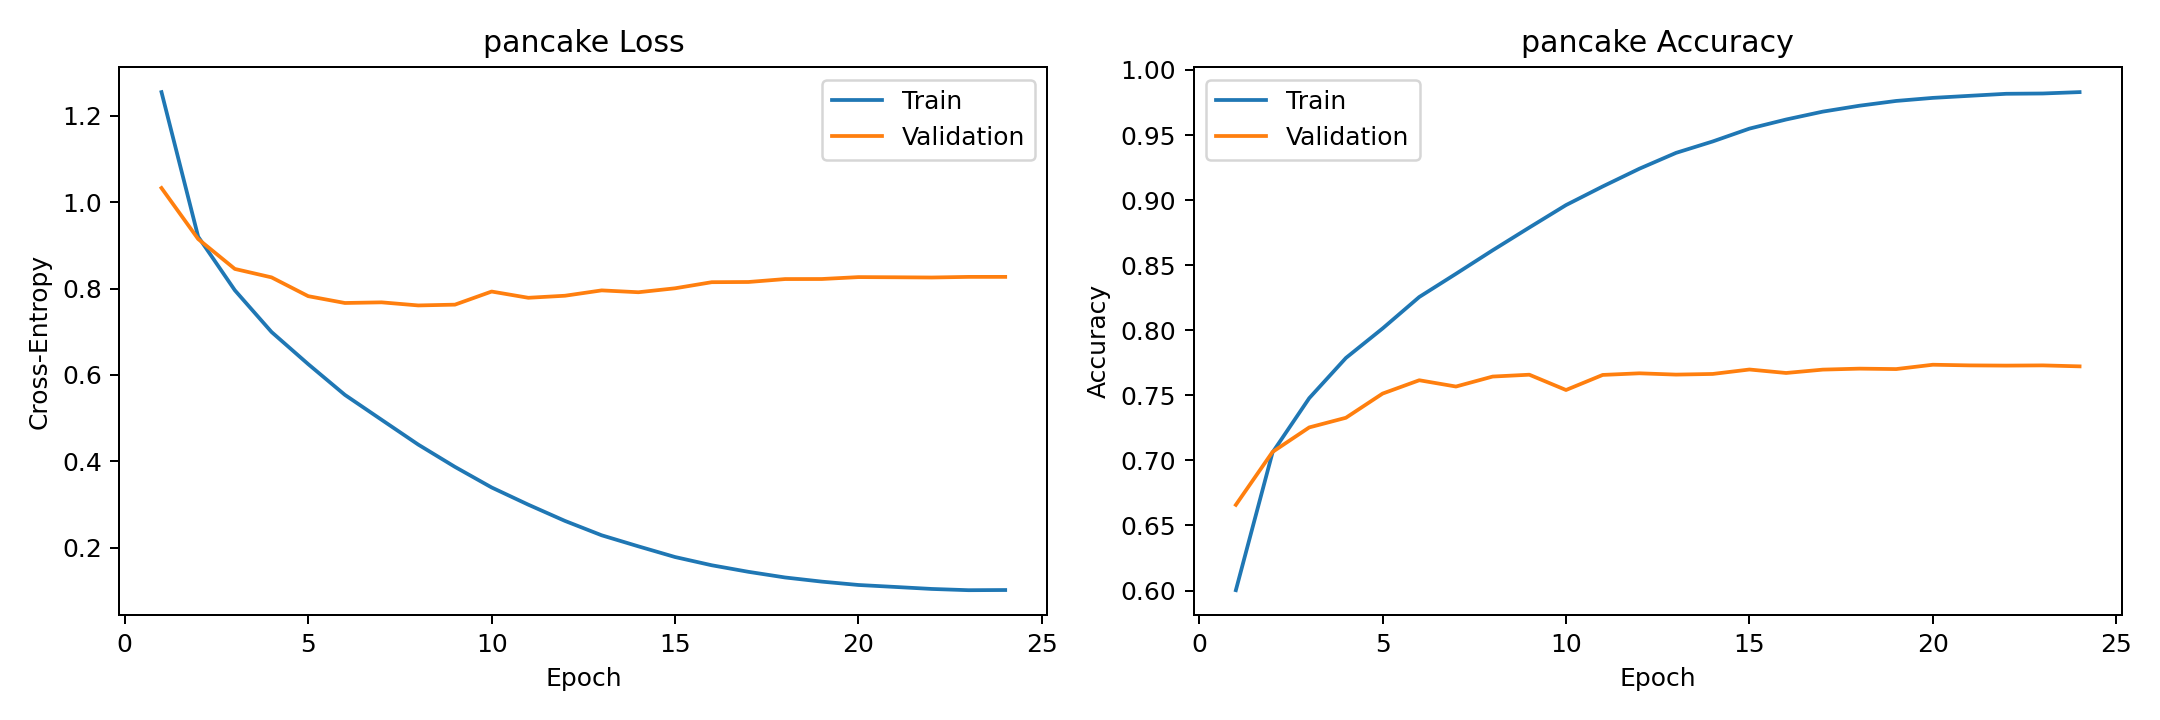
\includegraphics[width=\textwidth]{notebook_outputs/pancake_curves.png}
        \caption{Pancake curves}
    \end{subfigure}
    \hfill
    \begin{subfigure}[t]{0.48\textwidth}
        \centering
        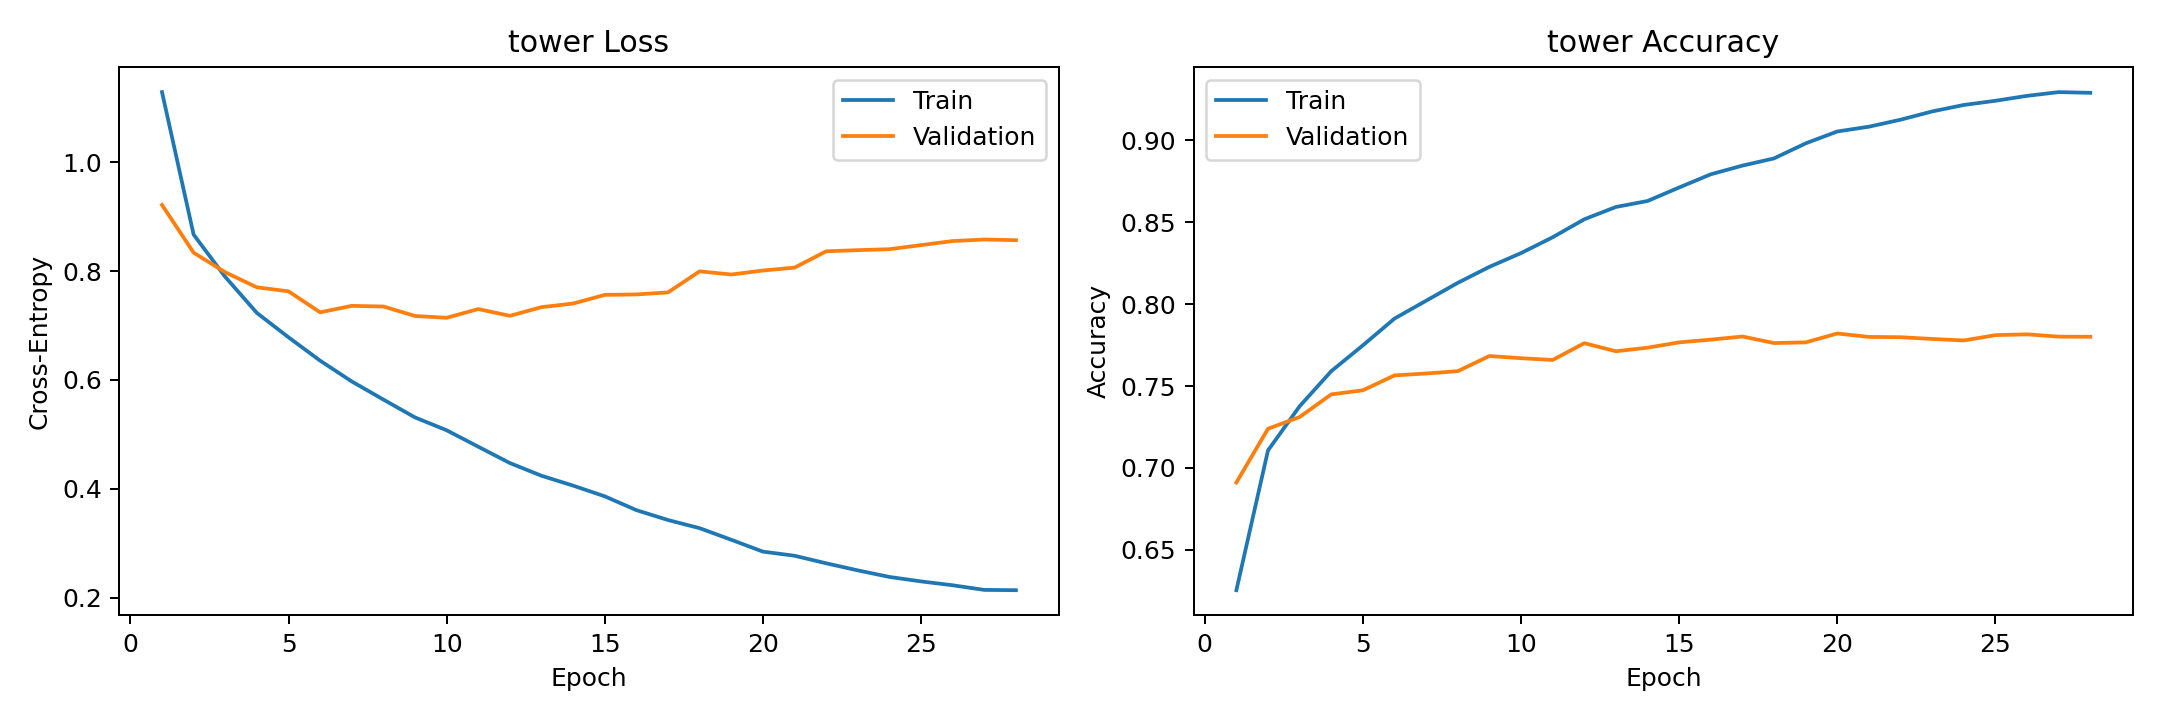
\includegraphics[width=\textwidth]{notebook_outputs/tower_curves.png}
        \caption{Tower curves}
    \end{subfigure}

    \vspace{0.5cm}
    \begin{subfigure}[t]{0.62\textwidth}
        \centering
        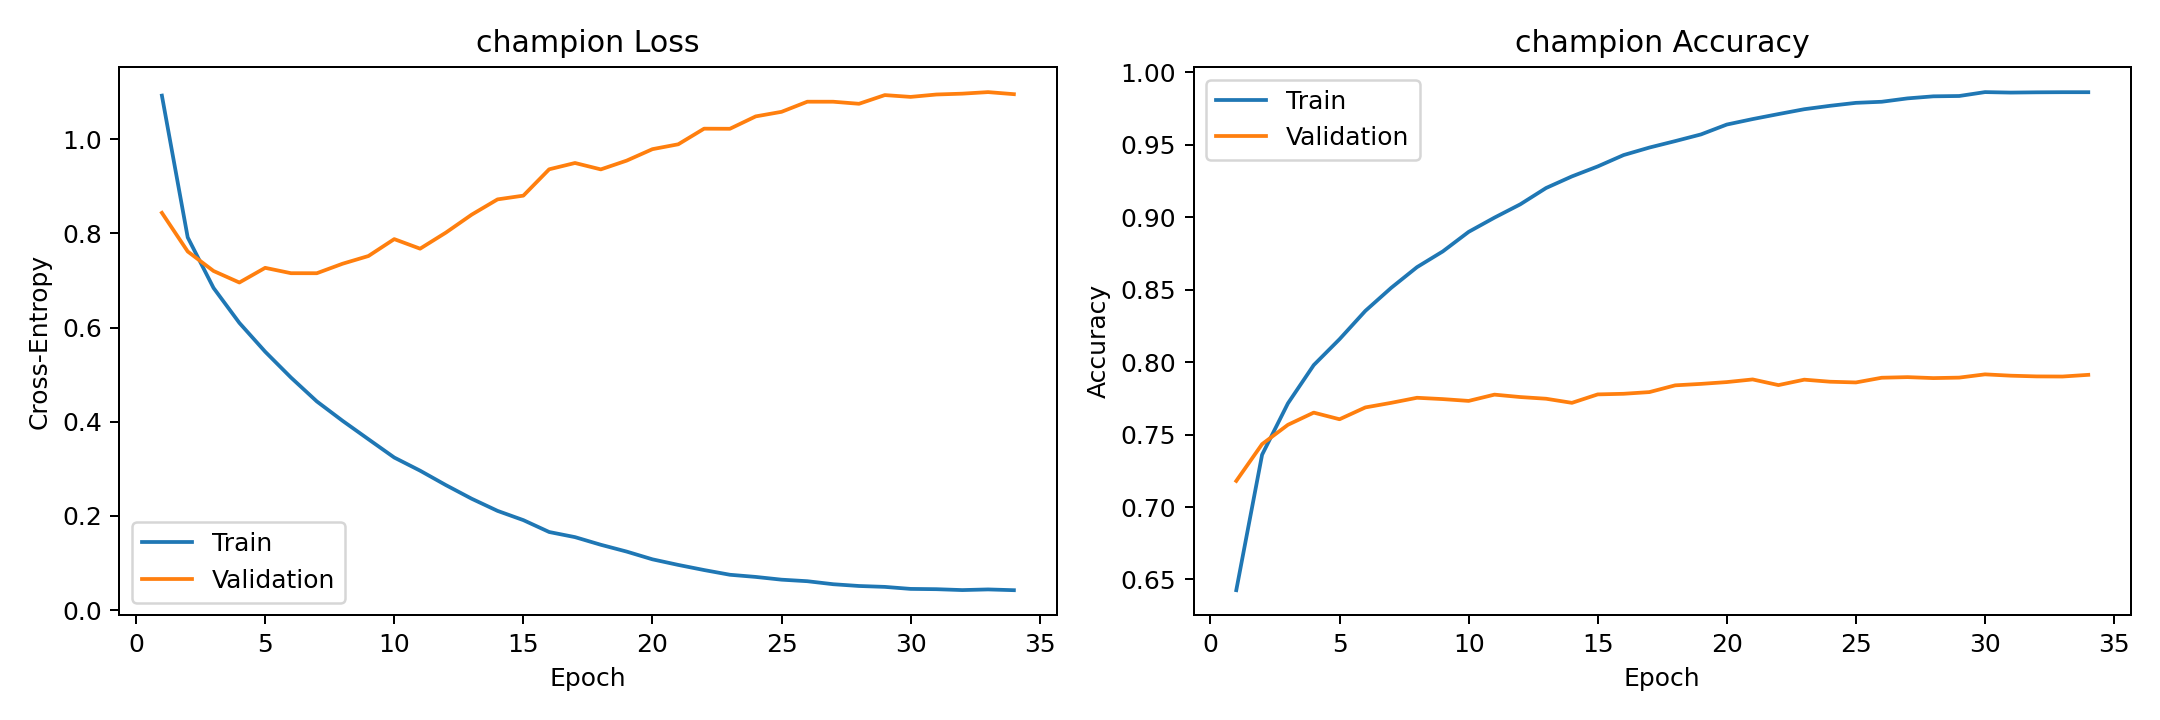
\includegraphics[width=\textwidth]{notebook_outputs/champion_curves.png}
        \caption{Champion curves}
    \end{subfigure}
    \caption{Training/validation loss and accuracy curves for all three models.}
\end{figure}

\section{Part D: Theoretical Analysis}
\subsection{D1. Width vs Depth}
The Universal Approximation Theorem states that a sufficiently wide single hidden layer can approximate any continuous function. However, in practice for image-like signals:
\begin{itemize}[leftmargin=1.5em]
    \item Deep networks learn hierarchical, compositional representations more efficiently.
    \item Depth often needs fewer parameters than an equivalent shallow model for comparable expressivity.
    \item Optimization and generalization are typically better when intermediate features can be reused over multiple layers.
\end{itemize}

From experiments:
\begin{itemize}[leftmargin=1.5em]
    \item Pancake: 1.64M params, 77.35\% validation accuracy.
    \item Tower: 0.54M params, 78.21\% validation accuracy.
    \item Champion: 2.13M params, 79.16\% validation accuracy.
\end{itemize}
This indicates that pure width is not sufficient; structured depth plus regularization improved validation performance.

\subsection{D2. Confusion Analysis}
\begin{figure}[H]
    \centering
    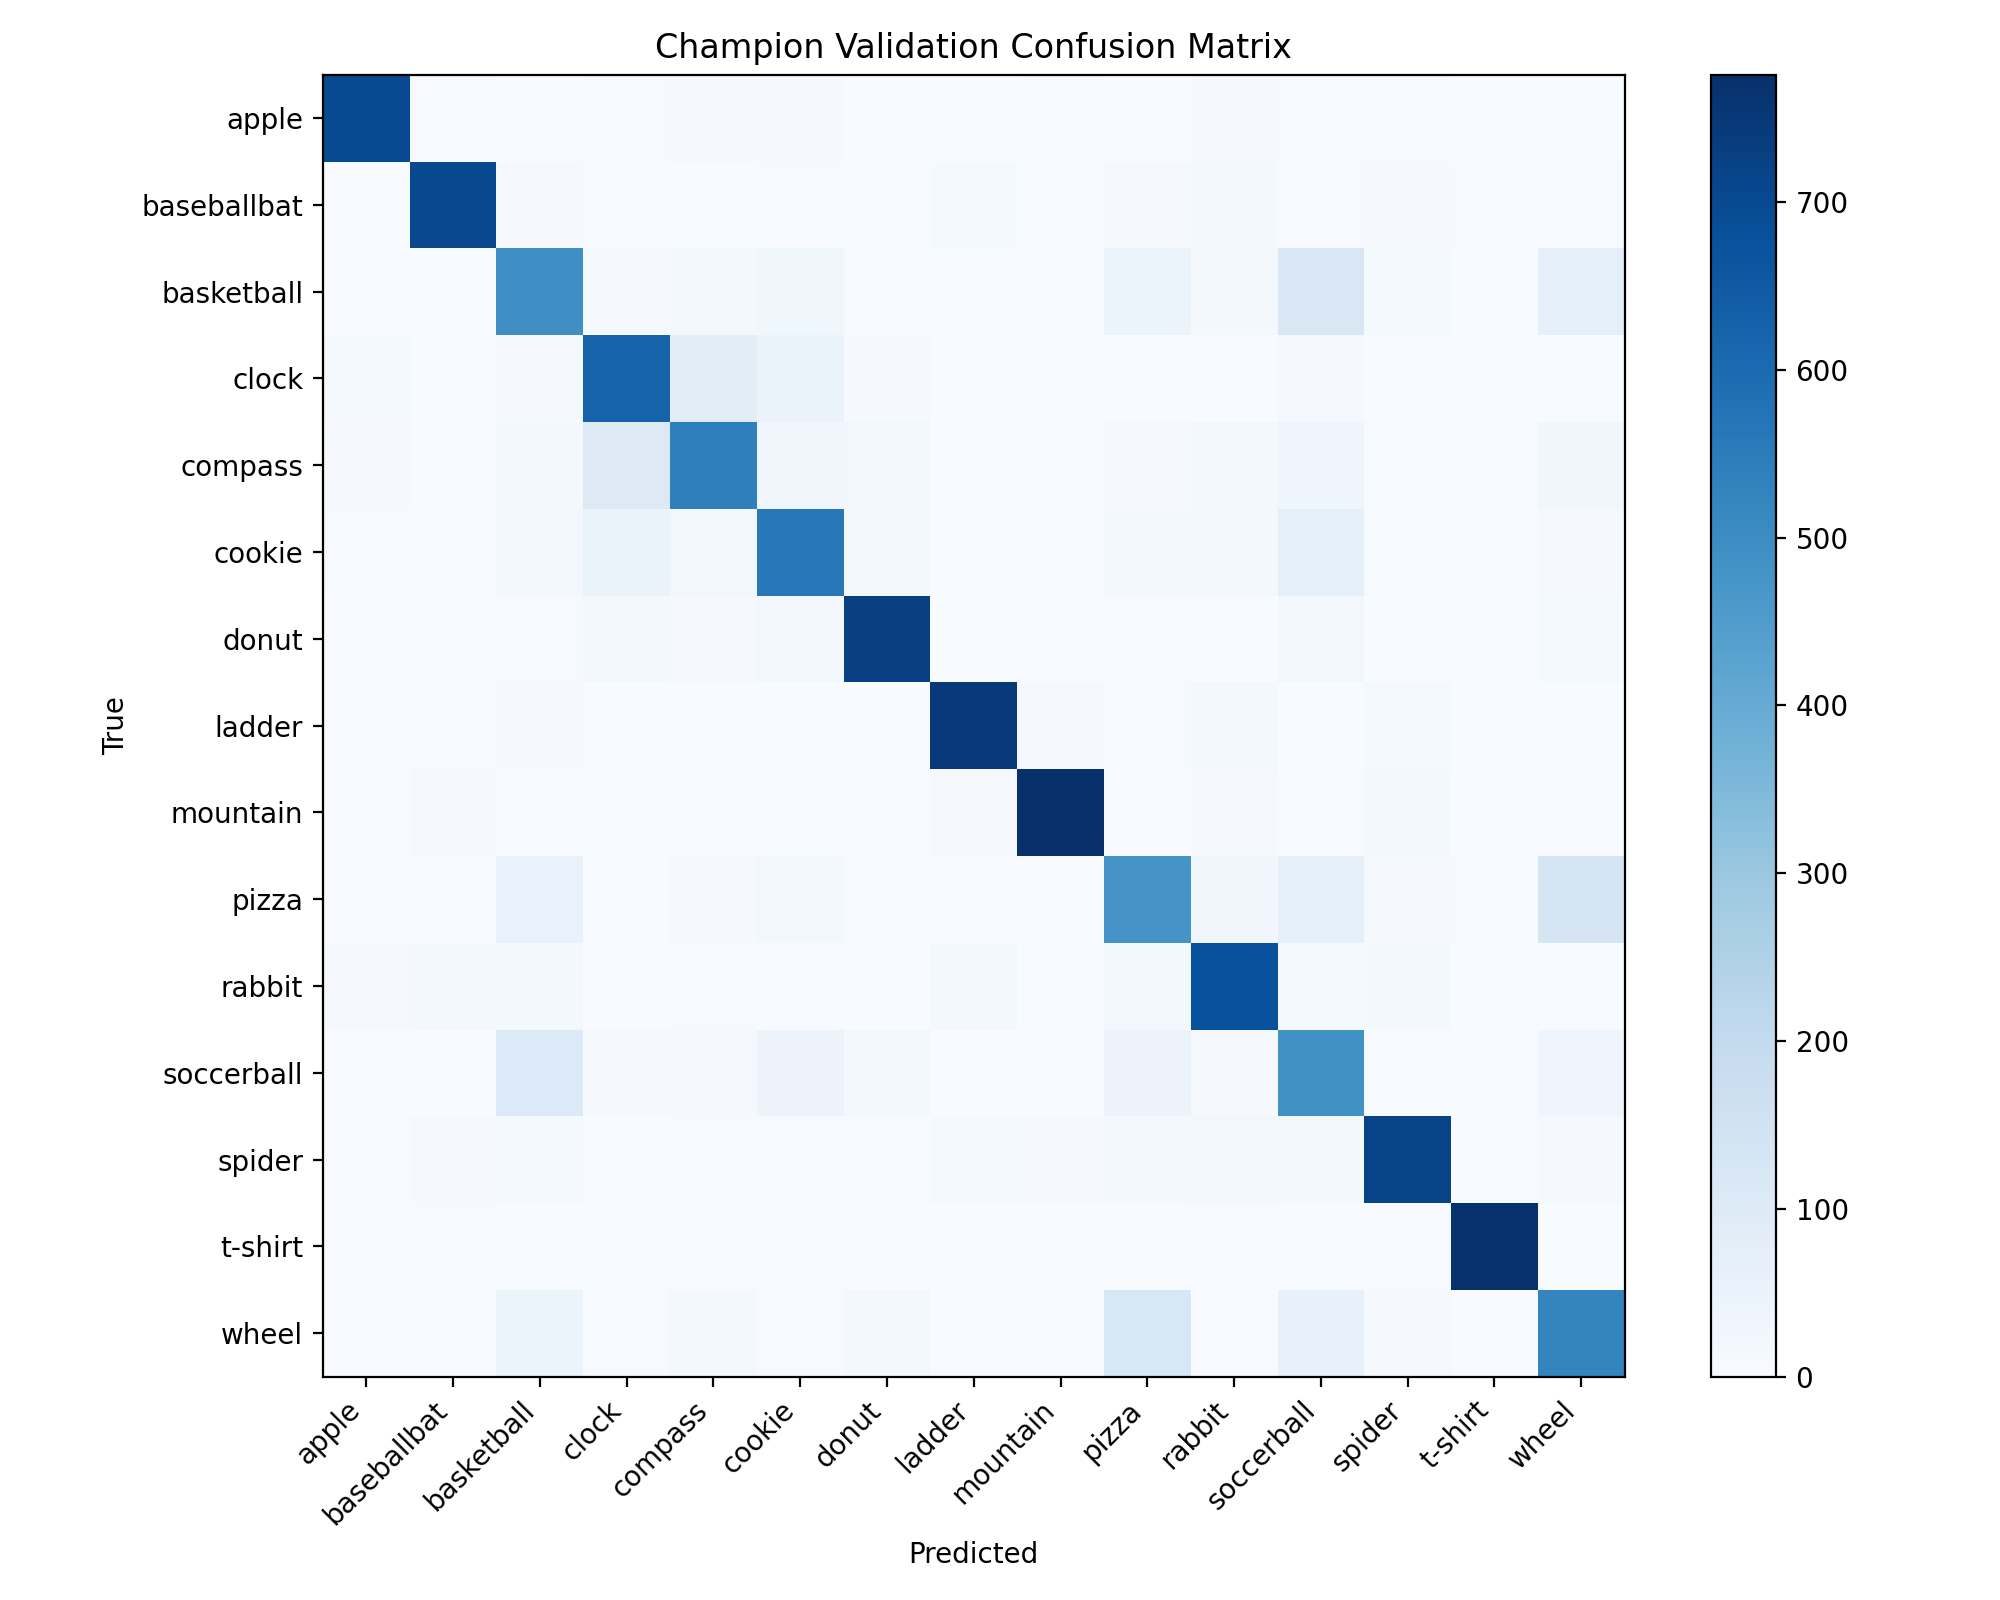
\includegraphics[width=0.84\textwidth]{notebook_outputs/champion_confusion_matrix.png}
    \caption{Confusion matrix of the selected champion model on local validation split.}
\end{figure}

Top-2 most confused class pairs:
\begin{enumerate}[leftmargin=1.5em]
    \item \textbf{pizza vs wheel}: 250 total confusions (pizza\(\rightarrow\)wheel: 129, wheel\(\rightarrow\)pizza: 121)
    \item \textbf{basketball vs soccerball}: 223 total confusions (basketball\(\rightarrow\)soccerball: 117, soccerball\(\rightarrow\)basketball: 106)
\end{enumerate}

\begin{figure}[H]
    \centering
    \begin{subfigure}[t]{0.48\textwidth}
        \centering
        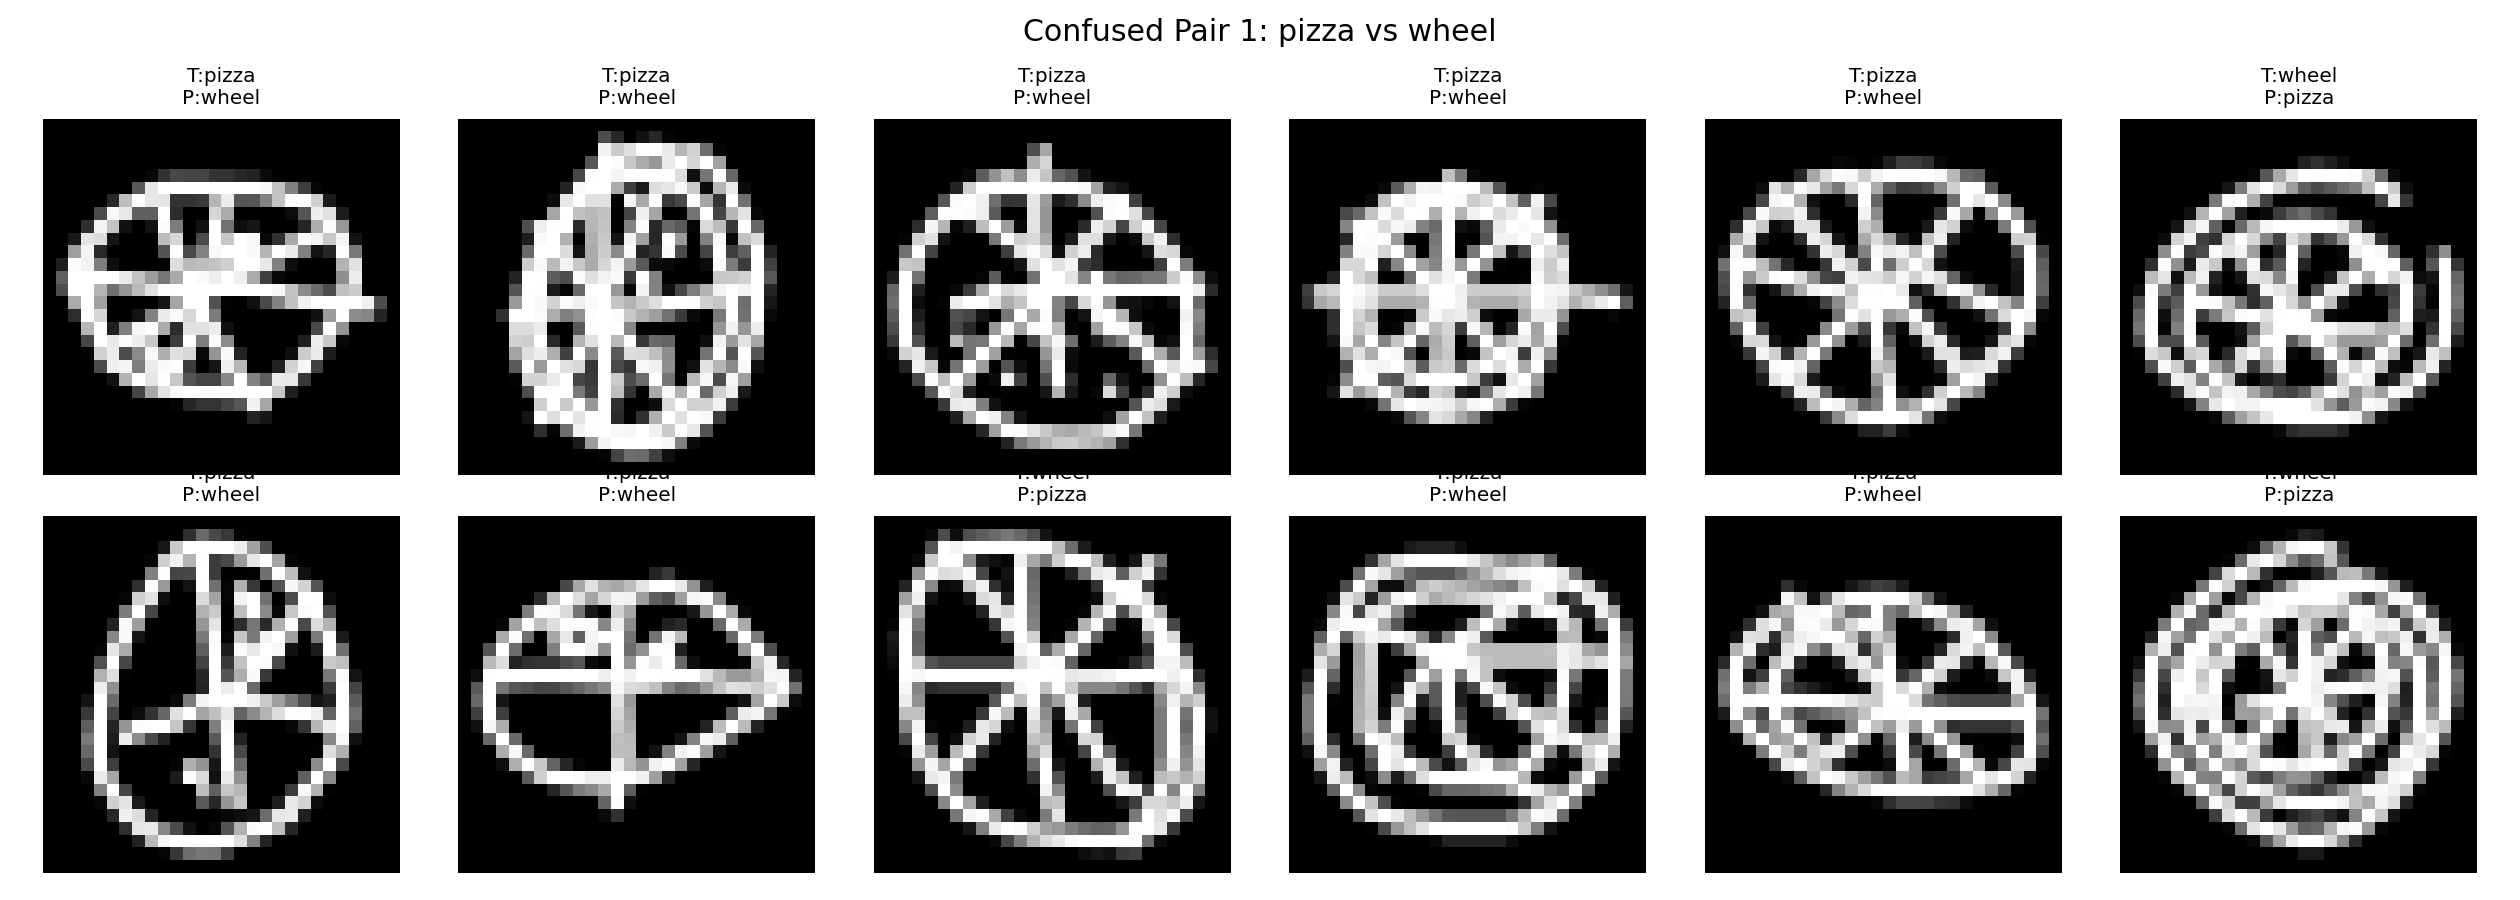
\includegraphics[width=\textwidth]{notebook_outputs/confused_pair_1_pizza_vs_wheel.png}
        \caption{pizza vs wheel}
    \end{subfigure}
    \hfill
    \begin{subfigure}[t]{0.48\textwidth}
        \centering
        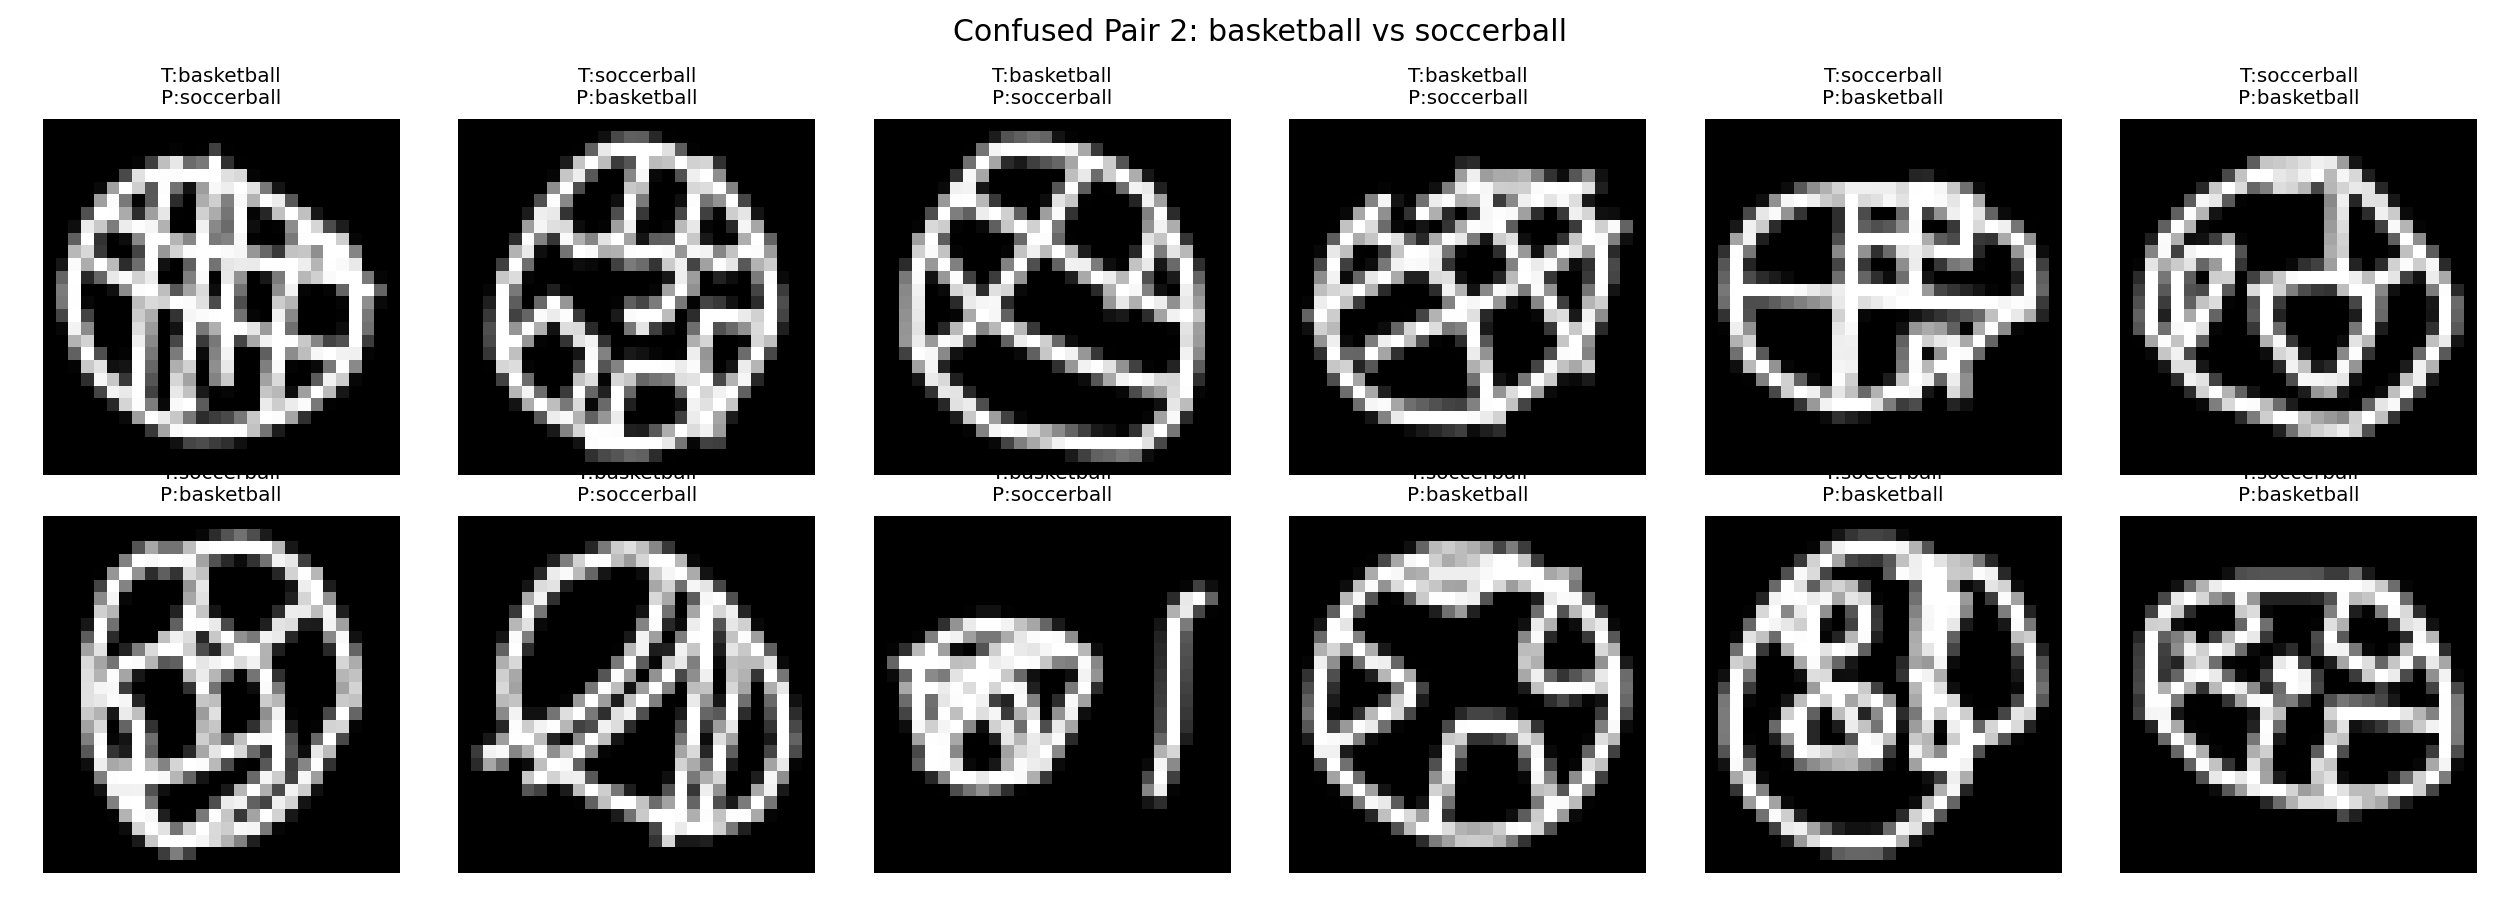
\includegraphics[width=\textwidth]{notebook_outputs/confused_pair_2_basketball_vs_soccerball.png}
        \caption{basketball vs soccerball}
    \end{subfigure}
    \caption{Visual examples from the two most confused class pairs.}
\end{figure}

\textbf{Interpretation:} A significant portion of these errors is due to \emph{aleatoric uncertainty} in human doodles (high intra-class variation and ambiguous sketches), though some residual model limitations remain.

\section{Part E: Architecture Rationale and Overfitting Control}
\subsection{Why this champion architecture?}
The champion uses a balanced depth-width profile ([1024, 768, 512, 256]) to improve expressivity while staying under the 3M parameter cap. It combines:
\begin{itemize}[leftmargin=1.5em]
    \item GELU activation for smoother nonlinear transitions.
    \item Batch normalization to stabilize deeper optimization.
    \item Dropout + weight decay to combat overfitting.
\end{itemize}

\subsection{Overfitting behavior}
Training curves show that training accuracy grows substantially higher than validation accuracy in later epochs, especially for wider models. This was mitigated using regularization and careful optimization choices.

\subsection{Final numbers for leaderboard form}
\begin{itemize}[leftmargin=1.5em]
    \item \textbf{Model Parameters:} 2,125,071
    \item \textbf{Epochs used:} 34
    \item \textbf{Predictions file:} \texttt{submission.txt} (comma-separated, 15,000 predictions)
\end{itemize}

\section{Reproducibility Artifacts}
Key files included in the repository:
\begin{itemize}[leftmargin=1.5em]
    \item Notebook: \texttt{<roll\_num>\_PA2.ipynb}
    \item Curves and analysis figures: \texttt{notebook\_outputs/*.png}
    \item Experiment summaries: \texttt{notebook\_outputs/model\_summary.csv}, \texttt{top2\_confusions.json}
    \item Champion checkpoint: \texttt{notebook\_outputs/champion\_best.pth}
    \item Leaderboard predictions: \texttt{submission.txt}
\end{itemize}

\section{Generative AI Usage Disclosure}
\textbf{Prompt used (summary):} Assistance was requested for structuring MLP experiments (Pancake/Tower/Champion), training pipeline design, confusion analysis workflow, and report drafting format.

\textbf{Generated output used:} Initial code/report structure suggestions and automation ideas.

\textbf{Edits made by student:} Dataset-specific adjustments, hyperparameter choices, architecture decisions, validation of outputs, and final report wording/organization were adapted for this assignment deliverable.

\vspace{0.5cm}
\noindent\textbf{Note:} The repository link above is the public submission repository for this assignment.

\end{document}
